\section{Biomass Carbon Storage and Removal}
BiCRS is a category of technologies which all use biomass as an input material to create negative emissions. The two most common technologies, Bioenergy with Carbon Capture and Storage (BECCS) and Biochar are considered in this thesis.

\subsection{Biomass availability}
Data about the global availability of waste biomass was collected from the FAOSTAT datasets on crops, livestock products and forestry \parencite{fao_faostat_2025, fao_faostat_2026}. The potential  of purpose-grown biomass was not considered in this model to avoid the issue of land competition, positioning the results on the conservative end of the range of potential estimates.\vspace{2mm}

For biomass from crop production, country-level FAO data for the production of crops was multiplied with the residue biomass generation factors from \textcite{lefebvre_biomass_2023}. The results covered 92.80\% of global crop production, while for the remaining 7.80\%, no residue factors were available. The results were subsequently multiplied with a collection factor of 30\% to account for the need to leave most of the residues in the field to avoid soil erosion and nutrient leech \parencite{battaglia_broad_2021}.\vspace{2mm}

For animal manure, a similar method was used. The country-level amount of livestock was collected from the FAOSTAT database, and multiplied with daily manure production and dry-mass collection factors from \textcite{lefebvre_biomass_2023}. These covered cattle, chicken, horses, sheep, goats, swine / pigs, making up 90.14\% of all global livestock.\vspace{2mm}

For forestry residues, the data from the FAO dataset on forestry was seperated into fuel wood and industrial wood (sawnwood). Based on an analysis by \textcite{koopmans_agricultural_1997}, it was assumed that logging residues would make up 1/3 of the raw wood cut down, and that 50\% of these residues could be harvested. For industrial woods, it was further assumed that another 50\% of the remaining 2/3 would turn into processing residues, all of which could be collected.

\subsection{Biomass cost}
The roadside cost (i.e. the cost to deliver the biomass residues to the roadside for pickup) was calculated based on biomass type and country. For crops, data from \textcite{bain_world_2007} was used to calculate a global, inflation-adjusted average cost, which was then adjusted for each country using purchasing power parity (PPP) data from the \textcite{world_bank_icp_2021}. For animal manure, a US-based handling cost of five US\$ per tonne was assumed, since manure is generally a waste product that holds little to no value and must be disposed of, and adjusted for PPP. Similarily, for forestry residues, a US-based price of 45 US\$ per tonne \parencite{skog_forest_2011} was adjusted for inflation and the country-level PPP factors. This resulted in the global marginal availability cost curve for waste biomass shown below. Note that this is a marginal availability cost curve for biomass, not a marginal abatement cost curve.
\begin{figure}[ht]
  \begin{center}
    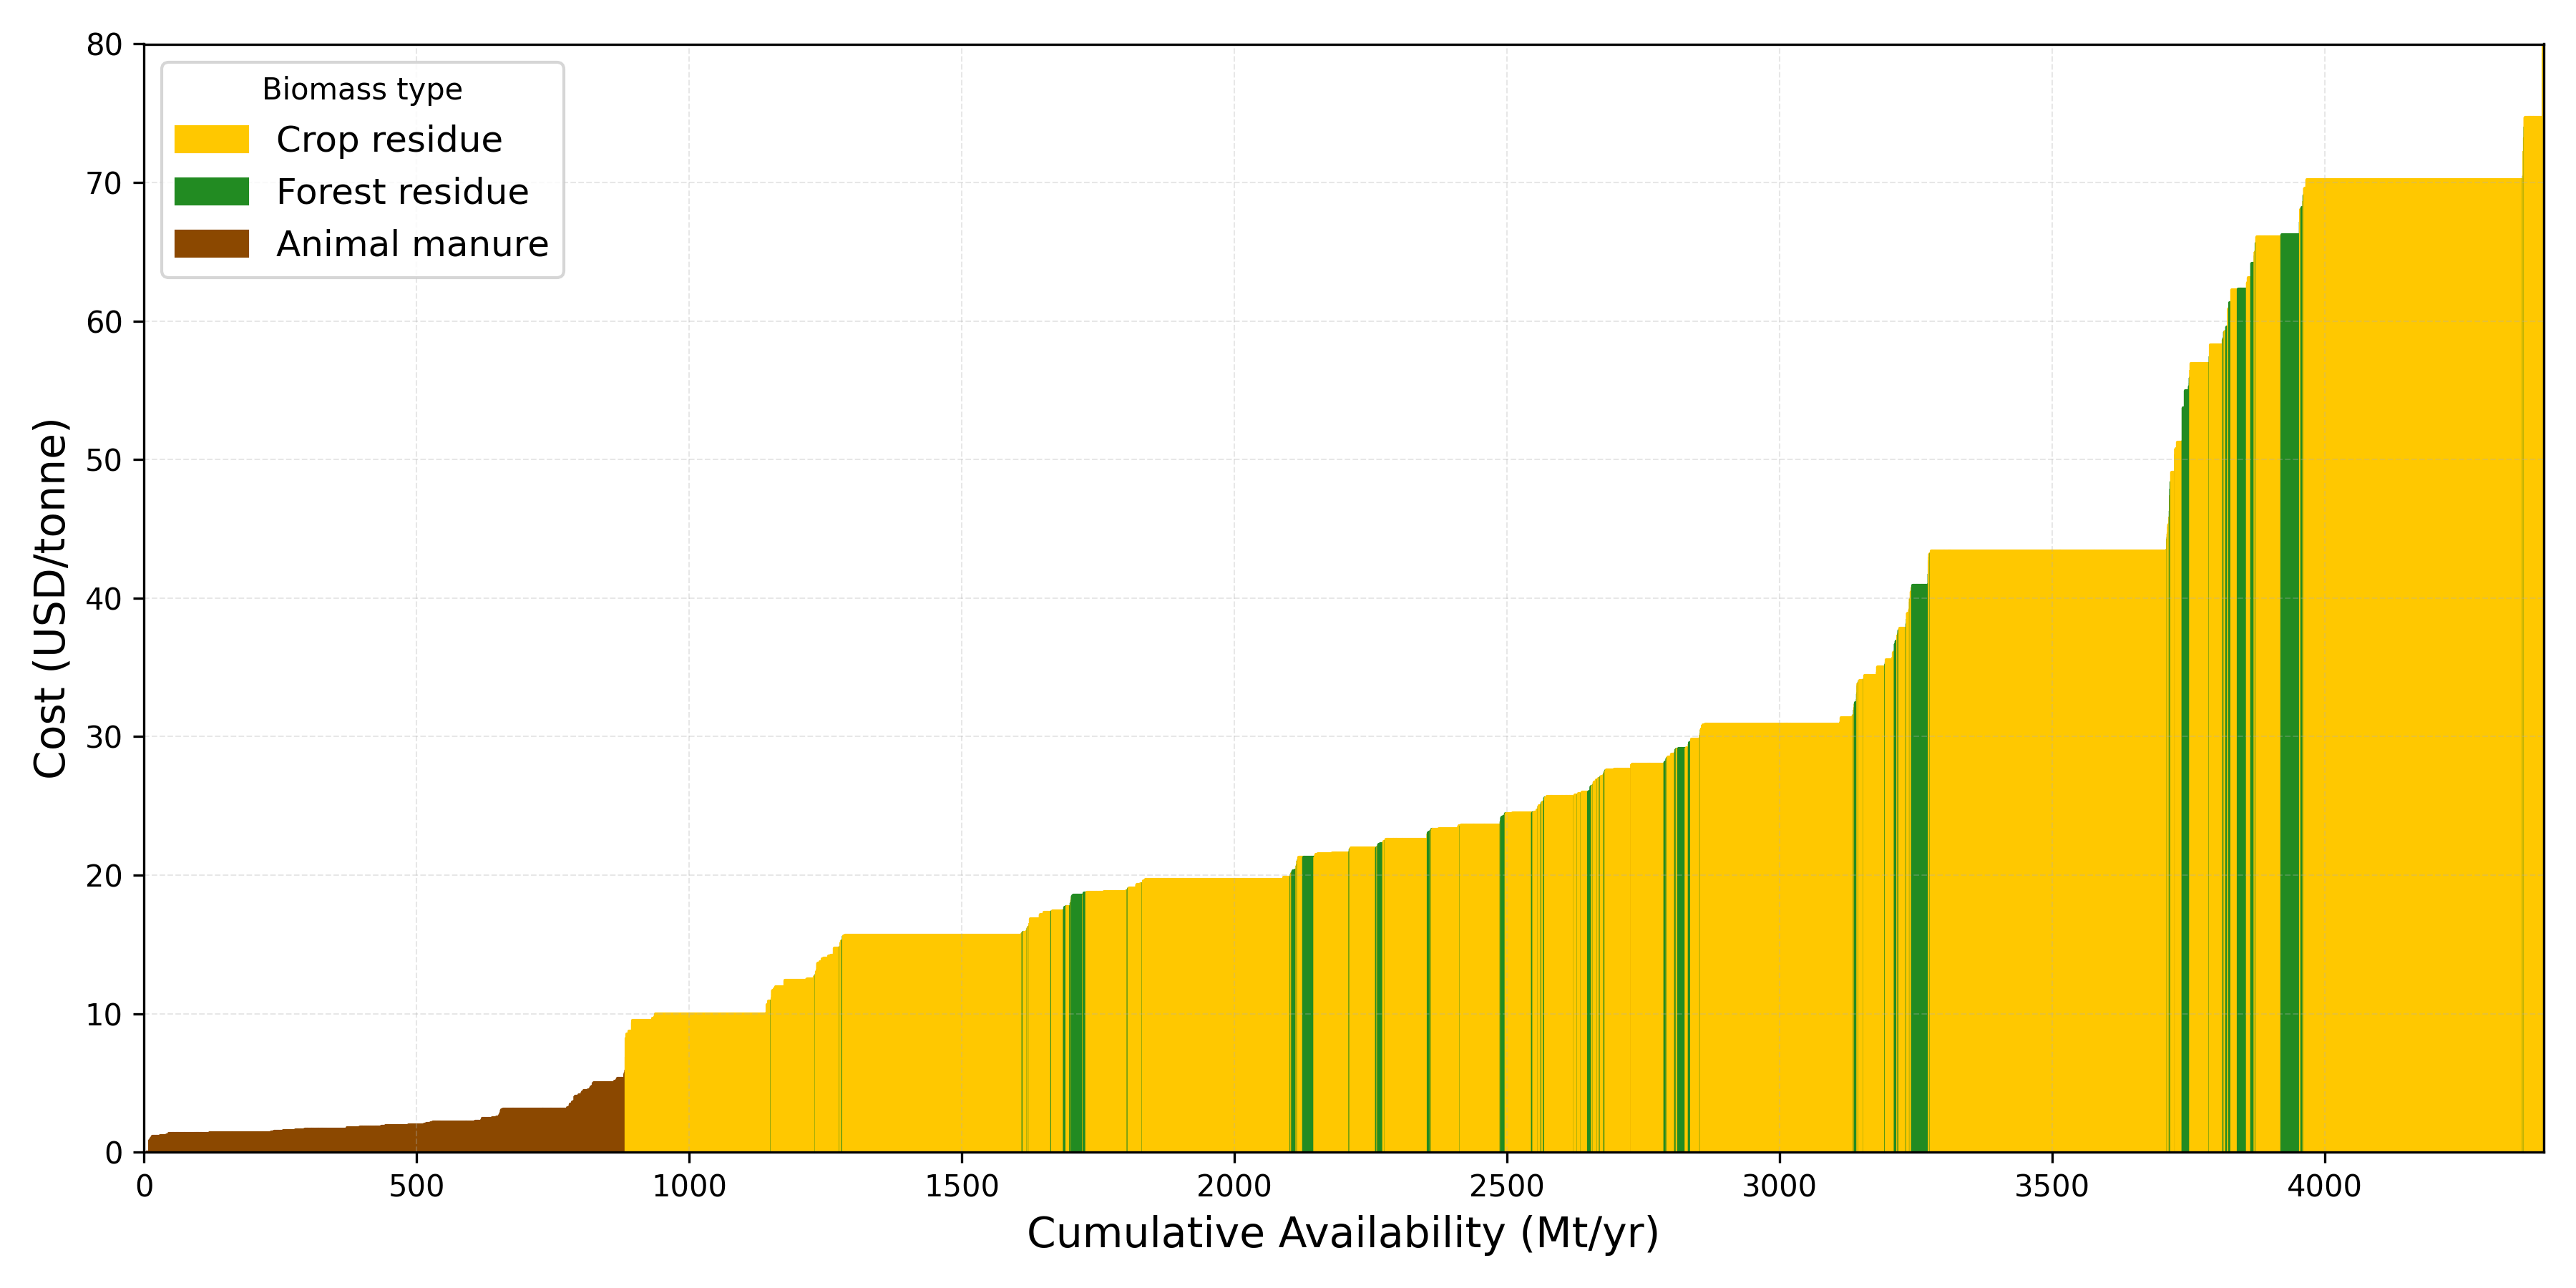
\includegraphics[width=1\linewidth]{figures/biomass_availability_chart.png}
    \caption{Global biomass marginal availability cost curve}
    \label{fig:biomass_mac_chart}
  \end{center}
  \vspace{-2em}
\end{figure}

\subsection{Bioenergy with Carbon Capture and Storage}
The BECCS model is based on an exemplary 250 MW biomass fired power plant. Assuming a capacity factor of 85\%, an annual energy output of about 1.4 GWh is generated.
\begin{wraptable}{l}{9cm}
\small
\renewcommand{\arraystretch}{1.3}
\begin{tabular}{llr}
\textbf{BECCS plant variables} &          &                \\ \hline
Total plant CapEx  & M\$       & 1875           \\
Total overnight cost & M\$       & 2254           \\
Gross capacity & MW       & 250            \\
Capacity factor & \%        & 85\%            \\
Gross annual output & MWh / yr & 1,861,500      \\
Auxilliary losses & \%        & 27\%            \\
Net annual output & MWh / yr & 1,358,895      \\
Efficiency factor & \%        & 21\%            \\
Required biomass & MWh / yr & 8,864,286      \\ \hline
\\
\end{tabular}
\caption{BECCS plant economic variables}
\end{wraptable}

To calculate the required amount of biomass, a 30\% baseline conversion efficiency for biomass combustion power plants is used and a 9\% penalty applied due to the use of CCS \parencite{cuellar_path_2015, fajardy_economics_2021}.\vspace{2mm}

For the calculation of the amount of carbon captured, the carbon content of each type of biomass is multiplied with an assumed capture rate of 90\%, and applied to the required input biomass amount. Finally, the co-revenues are calculated based on the sale of the generated net output energy at the applicable market rate. This method yields the hypothetical amount of biomass required, carbon captured, and revenues generated per year.\vspace{2mm}

The cost of the BECCS plant is based on capital expenditures and the annual fixed costs for operation and maintenance, primarily labor and material costs, as well as some variable costs such as non-fuel consumables and waste disposal. Similarly to the biomass costs, these too are adjusted for each country using the applicable PPP factor. To calculate the LCOC, all cost are annualized and divided by the amount of carbon removed. For the final LCOCR$^{+*}$, the transport and storage costs for CO$_2$ are added, the co-revenue of electricity sales is deducted, and a leakage factor of 24\% for transport and storage $\alpha_1$ is applied.\vspace{2mm}

By feeding the above biomass availability cost curve into this BECCS model, a global marginal abatement cost curve was constructed. It shows that BECCS using animal manure is generally the cheapest pathway, owed to the low assumed input costs. The overall LCOCR$^{+*}$ ranges from slightly below 100 US\$ (animal manure in low-cost countries) to around 210 US\$ (crop residues in high-cost countries).
\begin{figure}[ht]
  \begin{center}
    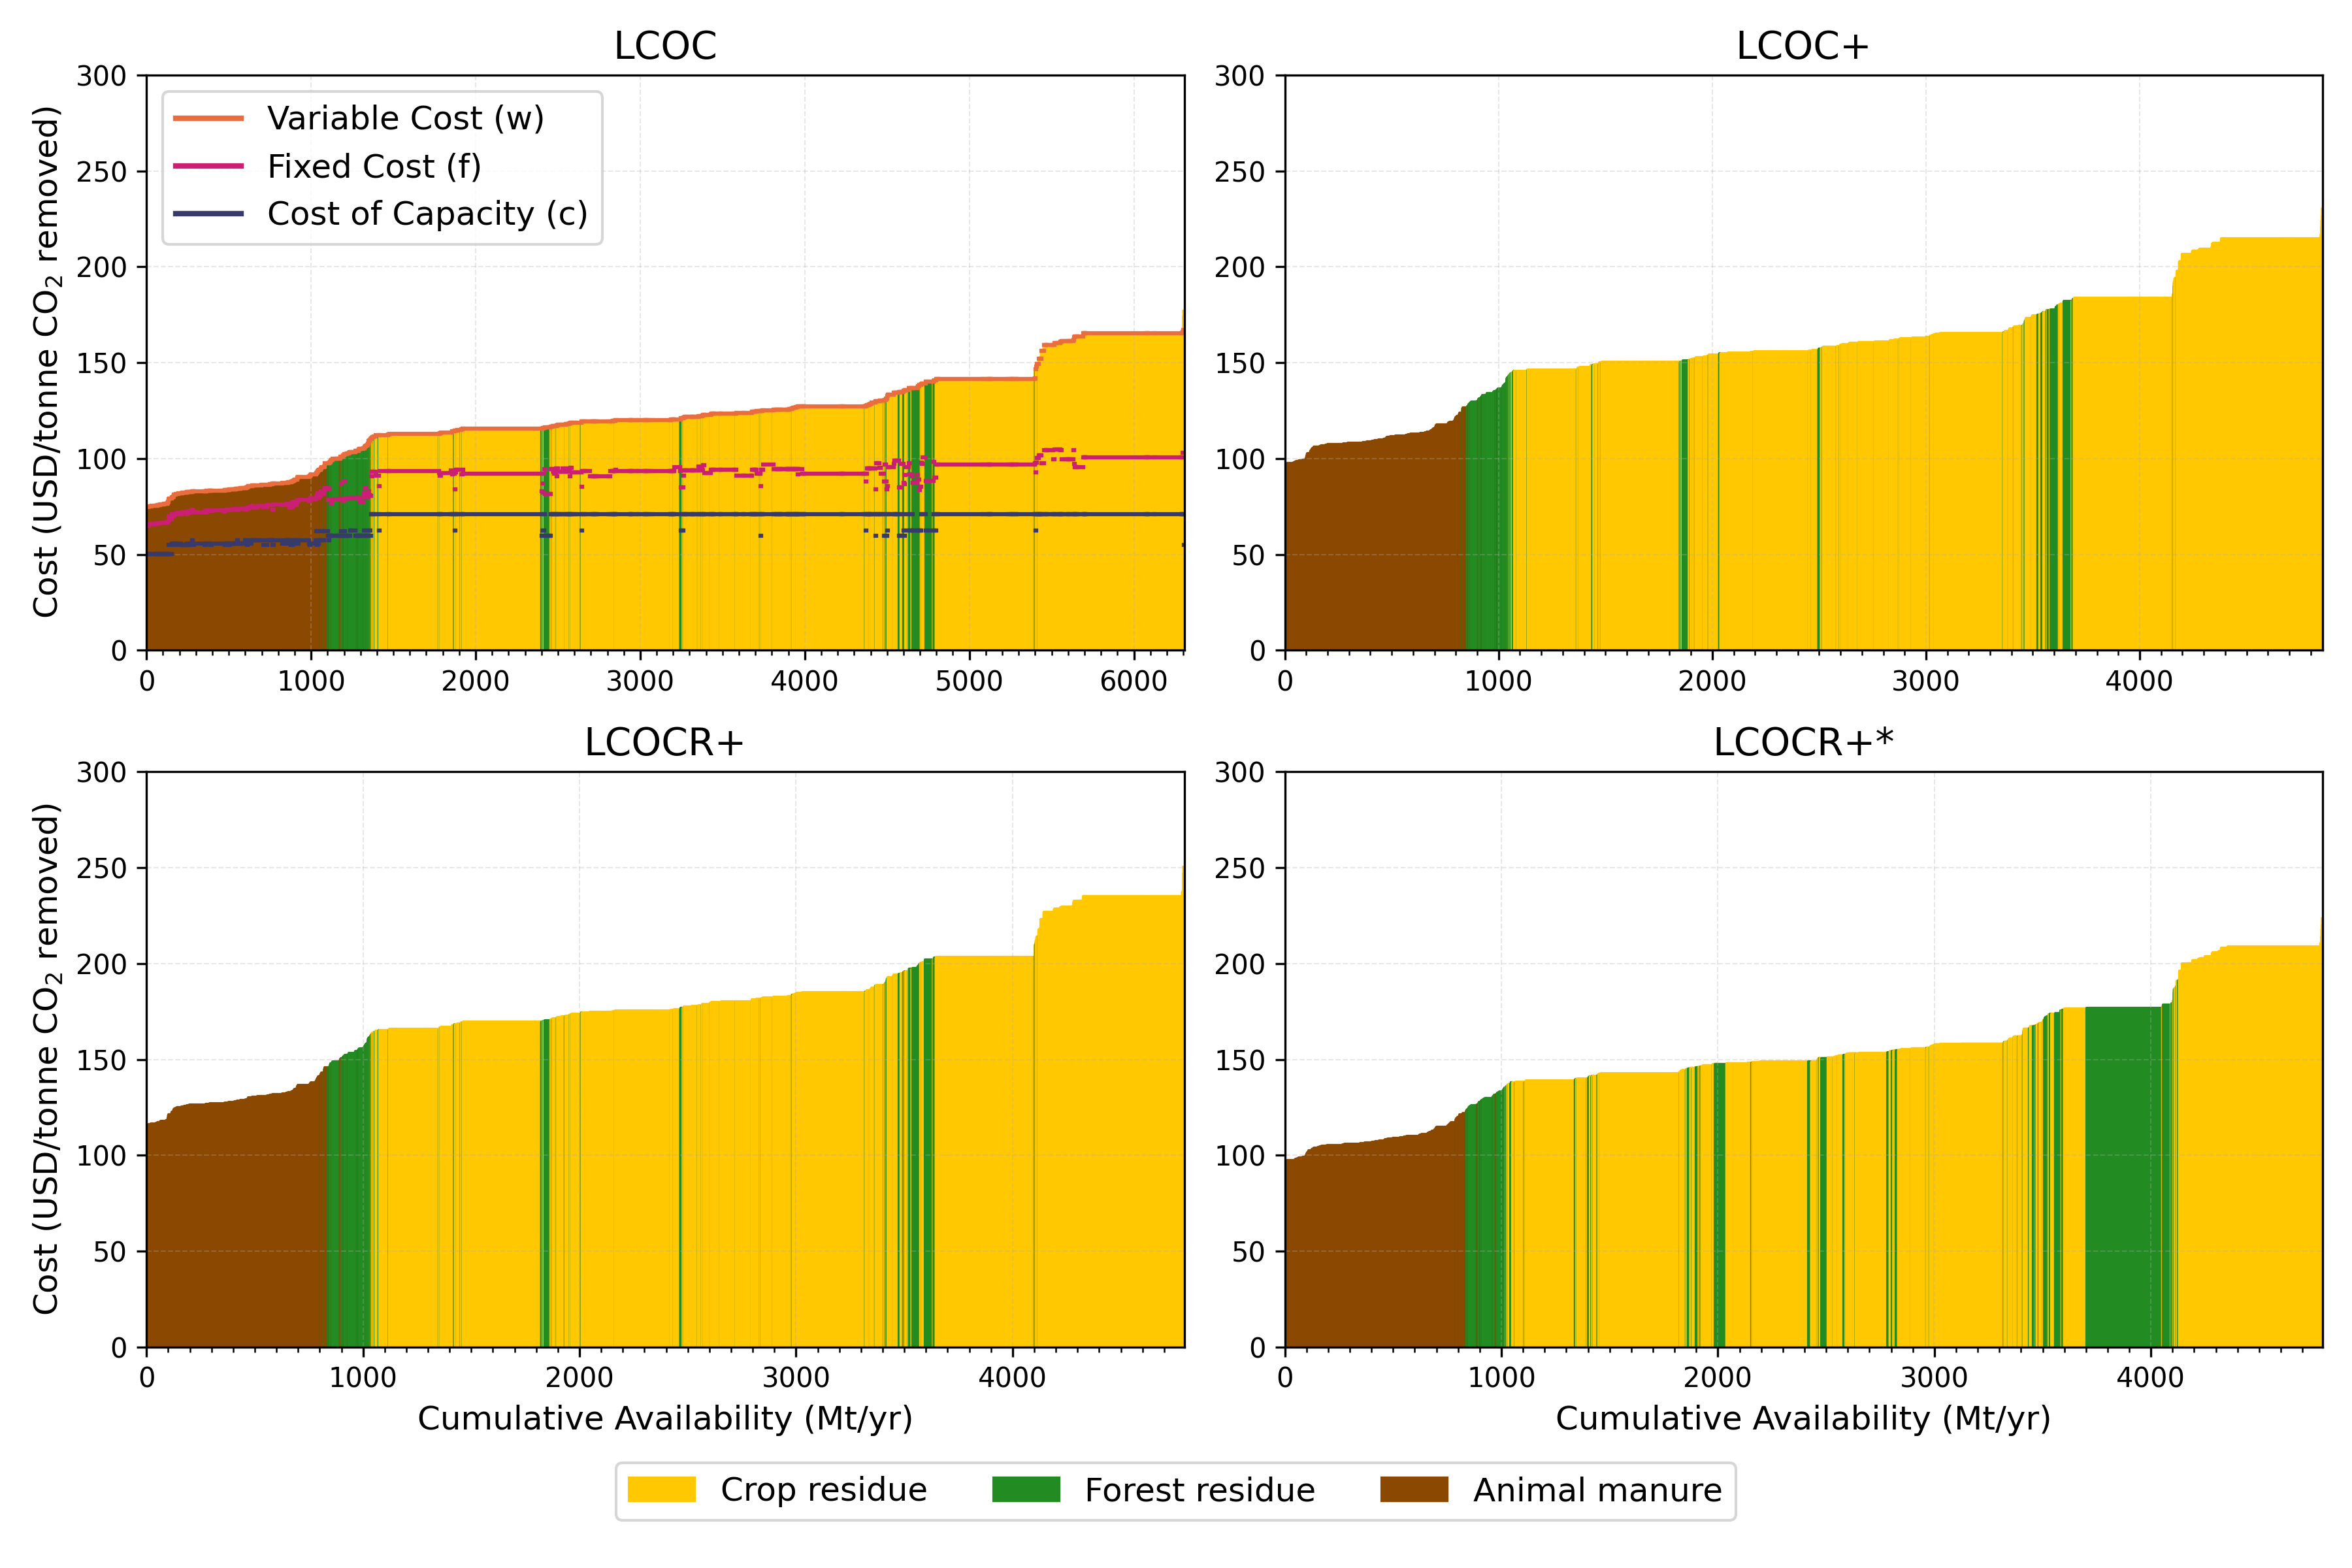
\includegraphics[width=1\linewidth]{figures/BECCS_macc_chart.png}
    \caption{Global BECCS marginal abatement cost curves}
    \label{fig:beccs_macc_chart}
  \end{center}
  \vspace{-2em}
\end{figure}

\subsection{Biochar}
Lorem ipsum...
